% ------- Create Preamble ------------
\documentclass [12pt]{article} 
\usepackage[a4paper]{geometry} 
\usepackage{amsmath, amsthm, amssymb, amsfonts}
 \usepackage{graphicx,epsfig}
\usepackage{booktabs} 
\usepackage{pslatex} 
\usepackage{caption} 
\usepackage{setspace} 
\usepackage{hyperref} 
\usepackage[noabbrev, nameinlink]{cleveref}
\usepackage{multicol, multirow}
\usepackage{graphicx,epsfig}
\usepackage{booktabs}
\usepackage{pslatex}
\usepackage{caption}
\usepackage{setspace}
\usepackage{hyperref}
\usepackage{multicol}
\usepackage{textgreek}
\usepackage{pdfpages}
\usepackage{apacite}
\usepackage{floatrow}
\usepackage{mdframed}
\usepackage{natbib} % For references
\bibpunct{(}{)}{;}{a}{}{,} % Reference punctuation
\def\citeapos#1{\citeauthor{#1}'s (\citeyear{#1})}
\newtheorem{hypothesis}{Hypothesis}
\newtheorem{nullhypothesis}{Null Hypothesis}
\usepackage{xcolor}
\hypersetup{
    colorlinks,
    linkcolor={blue!50!blue},
    citecolor={blue!50!blue},
    urlcolor={blue!50!blue}
}

\usepackage{booktabs}
\usepackage{siunitx}
\newcolumntype{d}{S[input-symbols = ()]}


\usepackage{lscape}
\usepackage{tikz}
\usetikzlibrary{shapes.geometric, arrows}
\tikzstyle{startstop} = [rectangle, rounded corners, minimum width=3cm, minimum height=1cm,text centered, draw=black, fill=white]
\tikzstyle{io} = [rectangle, rounded corners, minimum width=3cm, minimum height=1cm,text centered, draw=black, fill=white]
\tikzstyle{io2} = [rectangle, rounded corners, minimum width=3cm, minimum height=1cm,text centered, draw=black, fill=white]
\tikzstyle{arrow} = [thick,->,>=stealth]
%---Set up author and title page
\singlespace
\title{Snap judgements, emotion, and learning about politics}
\author{Damon C.\ Roberts\footnote{Ph.D Candidate,
Department of Political Science, University of Colorado Boulder, UCB 333, Boulder, CO 80309-0333. Damon.Roberts-1@colorado.edu.}}

%set up document
\date{\today}
\begin{document}
\maketitle


\newpage
\doublespace
\newpage
\section*{Introduction}

\begin{quote}
    ``All perceiving is also thinking, all reasoning is also intuition, all observation is also invention'' - Rudolf Arnheim
\end{quote}

Imagine we are at the airport and we see a bright red had with white lettering on it. You likely imagine a red hat with white lettering. You have well-trodden neurological paths of what the color red looks like, what a hat looks like, and what a hat with white lettering looks like. You are accessing associative memory to not just imagine what each of these things look like in isolation, but you likely have seen these things before. 

As this memory is associative, you likely have connected other things as well. Perhaps, you imagine that you are in the Dallas Airport. So you imagine the surroundings of the hat. You likely also imagine more than just the hat and it being in the Dallas Airport, but you likely imagine a wearer of the modal person wearing such a hat. From recency and contiguity, you likely associate such a hat with a white male who might be wearing cowboy boots (especially if you are in Texas).

Now you may feel negatively or positively about the hat and the wearer of the hat. The white lettering says something: ``Make America Great Again''. You know what political views this hat symbolizes. You likely have a valenced reaction to this individual wearing such a hat that has taken space in your imagination. You have a physiological reaction. Your heart rate increases, hands become clammy, or you may start finding yourself feeling enthusiastic with pulses of energy.

Visual information is a cognitively efficient means by which meaning is communicated. You are reading the prospectus of a dissertation from a political scientist. You sat down at your desk expecting to read something about politics. The first sentence tells you to imagine a red hat with white lettering on it. Rather than imagining the hat of an Arsenal F.C. fan, your mind jumped rather quickly to filling in more information about the hat and went right to one with political significance to Americans. The means by which this process occurs is of significant interest to those who examine the psychological foundations of learning and memory. While political psychologists have a rich literature on information processing and memory, much of it is conceptualized as a slower and more conscious process. This dissertation proposes a snap-judgement model of politically-relevant visual information to explain how individuals may pre-consciously detect, process, and appraise such information. 

The snap-judgement model asserts that it is visual information such as color and shapes that individuals rely on first to process politically-relevant information. From an evolutionary perspective, humans are attuned and adept at detecting and finding meaning from images. From a neurological perspective, processing visual information is much faster as it occurs simultaneously in different parts of the brain as opposed to text which takes a more linear path \citep{vogel_et-al_1986_wp}. Some estimates suggest that visual information can take as little as 13 milliseconds to be percieved \citep{potter_et-al_2014_app}. Visual information is not \textit{just} processed quicker, but it tends to have potency.

Visual information contains powerful meaning via affect. Visual information such as color contain important affective associations \citep{cimbalo_et-al_1978_jgp}. Memory associated with affect pass through the limbic system which mean that they are often easily and quickly encoded, easier to consolidate by placing it in an associative memory network, and will be easier to retrieve later \citep{kensinger_fields_2022_ohhum}.

Political symbology is common in politics and performs a significant role in shaping attitudes and behaviors. Strong partisans use yard signs as an expressive act which often succeed at generating valenced reactions from their neighbors \citep{makse_et-al_2019_oup}. Even in seemingly non-political ways, observing stereotyped cultural differences between Republicans and Democrats act as accurate visual cues (such as the modal car in the driveway) of any given neightborhood to make assumptions about the partisan composition of those who live there \citep{hetherington_weiler_2018_hmh}. Evidence suggest that Republicans like the ``Republican red'' more than they like the ``Democrat blue'' \citep{schloss_palmer_2014_pbr}. 

Connecting the literature on affective memory to existing work in political science on visual information yields the snap-judgement model. Going back to the example of the ``MAGA hat" exercise, the ``laws'' of recency, contiguity, and repitition \citep{kahana_et-al_2022_ohhum} would suggest that a simple prompt of red hat with white lettering would evoke a particular image. ``MAGA hats'' are a new but very prominent symbol representing the political views of the Trump-era Republican party. This means that it is easier to recall a ``MAGA hat'' than a hat with similar characteristics you may have seen years ago. With repitition, the connection is strengthened so that now, you are more likely to assume that I am describing a MAGA hat. As this visual information is encoded, so is the context. This means that when retreiving visual memories of a red hat with white lettering, contiguous neurological networks consolidating other visual information are retrieved as well. This means with memories of red hats with white lettering, you are more likely to recall other contextual information, e.g., the wearer of the hat and the meaning of the political views of those owning such a hat. As individuals have affective reactions to either congruent or incongruent political views \citep{iyengar_westwood_2015, druckman_levendusky_2019}, these memories should also be higher priority in that encoding, consolidiation, and retrieval should be easier than other neutral visual information \citep{kensinger_fields_2022_ohhum}. 

The snap-judgement model additionally expands upon extant theories of political information processing. The two leading theories of political information processing are \citeauthor{zaller_1992}'s \citeyearpar{zaller_1992} memory-based model and \citeauthor{taber_lodge_2006}'s \citeyearpar{taber_lodge_2006} online model. Both models present John Q. Public as a bayesian updater. The memory-based model presents JQP as one with a very weak prior that is amendable to change with new political information. The online model suggests that JQP heavily relies on their priors and will largely ignore new information that is not congruent with the prior. These models are agnostic to the type of information their models apply to. In their studies, the processing of such information is measured as conscious. Though, \citet{taber_lodge_2006} suggest that the making prior attitudes ``hot'' within about 800 milliseconds, it is still unclear what role snap judgements play. 

Fitting the snap-judgement model into the online model of information processing, it would suggest that these almost immediate appraisals should help one determine how one engages their attention. Information that activates retrieval for a particular memory tends to encourage attention when the associated affect is positive \citep{kensinger_fields_2022_ohhum}. This explains the tendency for individuals to perform poorly at recalling arguments by outpartisans \citep{lodge_et-al_1995}. 

Furthermore, it highlights a subsystem of information processing. Once an individual forms a snap-judgement, it their priors will take over and the affective reaction will activate a particular behavioral response. However, when incorrect appraisals or an intervening factor that attenuates the cognitive disengagement occurs, it may act as a valuable learning lesson that might have an opposite effect. As affective tagging of information can occur later \citep{kensinger_fields_2022_ohhum}, a positive experience despite a negative snap-judgement may weaken the association of a visual object with a negative affective response. Some evidence suggests that such a mechanism is plausible \citep{santoro_broockman_2022_sa}. As evidence suggests these depolarizing effects tend to be short term \citep{santoro_broockman_2022_sa}, the snap-judgement model suggests that this is due to the case that such interactions are not often reinforced so those memories are purged and the dampening effects are removed \citep[see][]{kahana_et-al_2022_ohhum}. It may be the case, however, that these are not all too common as individuals tend to avoid engaging with an object representing ideologically incongruent positions \citep[see][]{mutz_2006, klar_krupnikov_2016}.

\Cref{fig:snap-judgement_model} presents a summary of the snap-judgement model. This dissertation sets out to examine whether such a model exists. It will examine snap-judgements as prompted by a number of different types of visual information. The first empirical chapter will examine the speed at which individuals process such individual information by examining their attention to things like color on political yard signs. The second empirical chapter will step back to examine more complex visual information by asking participants to form snap judgements of a neighborhood with varying characteristics. The final empirical chapter will examine the implications of such a model on informal political discussions as they are often seen as a valuable opportunity to reduce affective polarization and to encourage democratic norms \citep{levendusky_stecula_2021, santoro_broockman_2022_sa}. 

\begin{figure*}
    \begin{mdframed}
    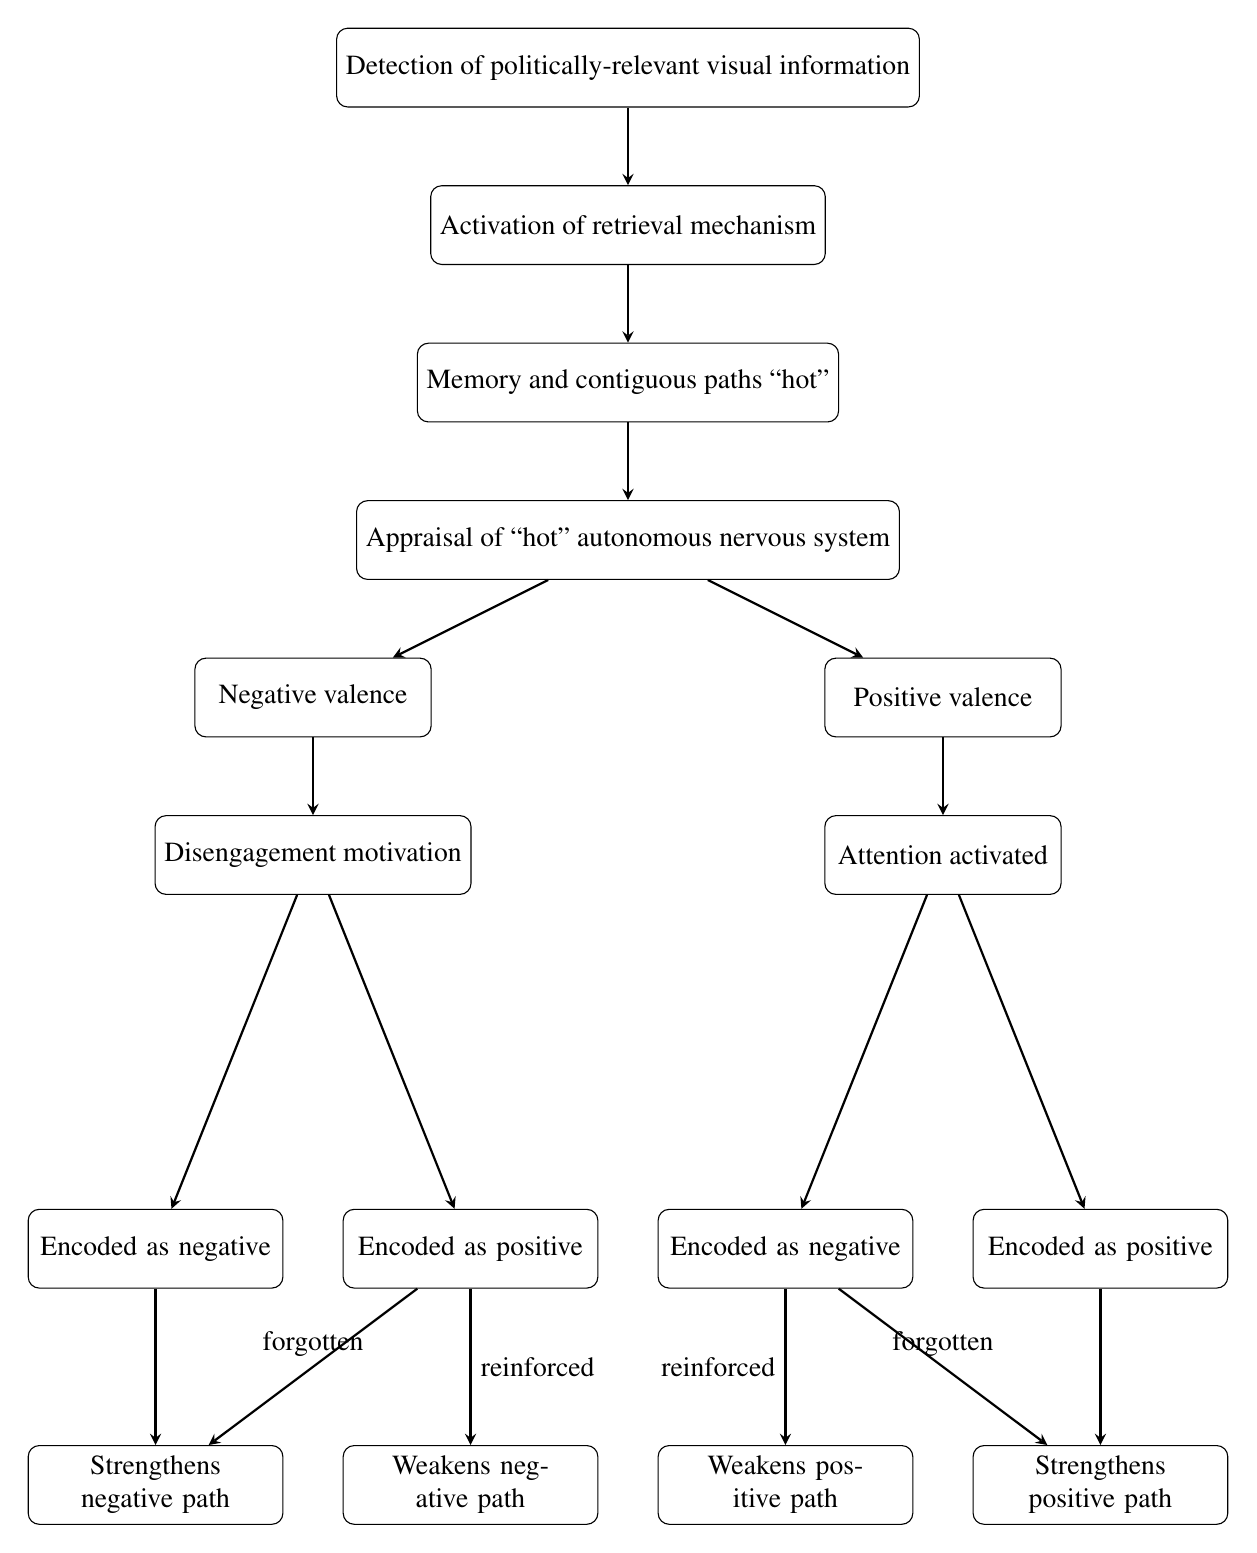
\begin{tikzpicture}[node distance = 2cm]
    \node (start) [startstop] {Detection of politically-relevant visual information};
    \node (in1) [io, below of=start]{Activation of retrieval mechanism};
    \node (in2) [io, below of=in1]{Memory and contiguous paths ``hot''};
    \node (in3) [io, below of=in2]{Appraisal of ``hot'' autonomous nervous system};
    \node (in4a) [io, right of= in3, xshift = -6cm, yshift = -2cm]{Negative valence};
    \node (in4aa) [io, below of=in4a]{Disengagement motivation};
    \node (in4aaa) [io, below of=in4aa, xshift = -2cm, yshift = -3cm, text width = 3cm]{Encoded as negative};
    \node (in5ns) [io, below of=in4aaa, yshift = -1cm, text width = 3cm]{Strengthens negative path};
    \node (in4aab) [io, below of =in4aa, xshift = 2cm, yshift = -3cm, text width = 3cm]{Encoded as positive};
    \node (in5nw) [io, below of =in4aab, yshift = -1cm, text width = 3cm]{Weakens negative path};
    \node (in4b) [io, left of=in3, xshift = 6cm, yshift = -2 cm]{Positive valence};
    \node (in4ba) [io, below of =in4b]{Attention activated};
    \node (in4baa) [io, below of=in4ba, xshift = -2cm, yshift = -3cm, text width = 3cm]{Encoded as negative};
    \node (in5pw) [io, below of = in4baa, yshift = -1cm, text width = 3cm]{Weakens positive path};
    \node (in4bab) [io, below of=in4ba, xshift = 2cm, yshift = -3cm, text width = 3cm]{Encoded as positive};
    \node (in5ps) [io, below of=in4bab, yshift = -1cm, text width = 3cm]{Strengthens positive path};
    \draw [arrow] (start) -- (in1);
    \draw [arrow] (in1) -- (in2);
    \draw [arrow] (in2) -- (in3);
    \draw [arrow] (in3) -- (in4a);
    \draw [arrow] (in4a) -- (in4aa);
    \draw [arrow] (in4aa) -- (in4aaa);
    \draw [arrow] (in4aaa) -- (in5ns);
    \draw [arrow] (in4aa) -- (in4aab);
    \draw [arrow] (in4aab) -- node[anchor =west]{reinforced}(in5nw);
    \draw [arrow] (in3) -- (in4b);
    \draw [arrow] (in4b) -- (in4ba);
    \draw [arrow] (in4ba) -- (in4baa);
    \draw [arrow] (in4baa) -- node[anchor = east]{reinforced}(in5pw);
    \draw [arrow] (in4ba) -- (in4bab);
    \draw [arrow] (in4bab) -- (in5ps);
    \draw [arrow] (in4aab) -- node[anchor = south]{forgotten}(in5ns);
    \draw [arrow] (in4baa) -- node[anchor = south]{forgotten}(in5ps);
\end{tikzpicture}
\end{mdframed}
    \caption{Snap-judgement model of politically-relevant visual information}
    \label{fig:snap-judgement_model}
\end{figure*}

%What image does this evoke? Do you see just the hat? Do you have memories which suggest that you should associate such visual information with other information? Do you imagine the wearer of the hat being a man, being white, perhaps even wearing cowboy boots? Do you now think you are at an airport in New York City or at an airport in Dallas Texas? Do you know what the message on the hat in white lettering says? Perhaps it says "Make America Great Again". What physical reaction do you have to this image? Perhaps your heart rate increases, perhaps your hands become a bit clammy. Do you feel disgusted, angry, excited? How quickly did you conjure such an image in your mind? How quickly did different parts of that image form? Did the hat and the features of the wearer come faster than the text on the hat and faster than imagining a particular airport? Did you anticpate that the hat was a symbol for a political message?
%
%Visual information is quite powerful. Symbols and visual information conveying a story or ideas have a much deeper root in human evolution than written text. Our brains are optimized to percieve and to associate visual information with memories at remarkable rates. Some estimate that the processing of visual images happen in as little as 13 milliseconds \citep{potter_et-al_2014_app}. Text-based information happens much slower as it follows a linear and ordered process through the brain unlike visual information which can be processed simultaneously in different regions of the brain \citep{vogel_et-al_1986_wp}.
%
%As visual information is efficient, it has an important place in politics. Symbols and colors that represent parties, countries, and ideologies are readily recognizable. The first televised presidential debate is said to be a turning point in the campaign of a young and attractive John F. Kennedy. Yard signs with the name of a political candidate are put up by strong partisans as an expressive act which often succeed at generating valenced reactions from their outpartisan neighbors \citep{makse_et-al_2019_oup}. Even in seemingly non-political ways, observing stereotyped cultural differences between Republicans and Democrats act as accurate visual cues (such as the modal car in the driveway, or whether it is a suburb or densely populated, mixed use neighborhood) of any given neighborhood to make assumptions about the partisan composition of those who live there \citep{hetherington_weiler_2018_hmh}. This work among political psychologists has yet to unpack the particular mechanism by which visual information works in associative memory to take both political and seemingly apolitical information to shift attitudes and behavior. Moreover, as visual information is a much more efficient source than text, it has yet to be studied how it is a more effective means by which people come to accurate and rapid politically-relevant appraisals with only visual information.
%
%This dissertation studies the role of visual information in producing snap judgments about others in reference to their political views. In doing so, I argue that visual information produces faster and stronger affective responses than text-based information. Using an affective memory and hot cognition model, it argues that politically-relevant visual information is encoded as affectively charged in long-term memory. With new political information sparking associative memory, this new visual information is quickly percieved and brought to consciousness along with prior associated memories and their valenced charge. As this information reaches consciousness first, visual information produces a quick, gut-level, and affective snap judgement about the image. 
%
%The implications of such a theory inform not only the way in which political information is processed, but more importantly it identifies the foci. As previous research on political memory and information processing has debated the way in which individuals access and store new political information, the preeminant memory \citep{zaller_1992} and online models \citep{lodge_et-al_1995} of information processing characterize new information as complete and wholistic. Acting within a subsystem, a snap judgement based only on visual information produces an almost immediate barrier if one pre-consciously associates this visual information with negative valence. In taking this view, this model of snap judgements relies on the theory of affective intelligence which suggests that distinctive categories of affect encourage distinctive behaviors.
%
%The model suggests that snap judgements that call particular affectively encoded associative memories influence the degree to which one consciously engages with the new information. Where visual information activates affectively charged associative memories that suggest retreat, the model suggests that attempts to shift foci on other features are less likely. This necessarily means that visual information that activates affectively charged associative memories that suggest approach, will encourage an individual to shift their focus on other features and to engage in conscious processing are more likely. 

%Information is affectively encoded. Early work in psychology demonstrates that visual information often has affective attatchments \citep{cimbalo_et-al_1978_jgp}. These associations with visual information and affect are likely learned. The theory of hot cognition suggests that we rarely learn information through details but rather we can speed up this process through encoding this information \textit{vis-a-vis} affect. As a theory of memory encoding, hot cognition is believed to be important for the processing of political information and the formation of political attitudes \citep[see][]{taber_lodge_2006_cup}. Once stored in long-term memory, this information can be accessed later through similarity which trigger similar neurological patterns.

%We use visual information to make judgements about others. We seek to understand who they are just by the way they dress, the way they carry themselves, and the way they take up space. These features are also expressive. We curate the way we visually present ourselves as a way to represent to our personality. To percieve visual information light passes from the cones and rods in our eyes to our optical nerve, then to our lateral geniculate nucleus in the thalamus to our visual cortex. Once percieved, visual information passes through our brain to spark memories and to reinforce others. Some estimate that the processing of visual images happen in as little as 13 milliseconds \citep{potter_et-al_2014_app}. While it takes longer to connect this information to memory and even consciousness, visual information is powerful and fast. But just how useful are these fast sources of information for understanding politics?
%
%The advent of televised Presidential debates partly contributed to the success of a young and attractive, John F. Kennedy. Some political psychologists connect the role of visual information as a source of political information. \citet{hetherington_weiler_2018_hmh} demonstrate that individuals are able to accurately attribute the partisan leanings of a given neighborhood only with visual information that communicates cultural stereotypes that differ between partisans. \citet{makse_et-al_2019_oup} demonstrate that strong partisans tend to put up yard signs as an expressive act which tend to produce strong valenced reactions among outpartisan neighbors. What remains unclear in such narratives is whether these sources of visual information produce ``snap judgments'' and what the implications of such evaluations have on learning and social interactions.
%
%Politically-relevant information is encoded in long-term memory with the help of emotion. \citet{lodge_et-al_1995} demonstrate that individuals do not store the details of political information in long-term memory, but rather that they encode it as valanced information. This information is accessed through hot cognition, a mechanism whereby this information is stored based upon affectively-charged information. This information is most accessible when similar affectively charged information reminds one of it \citep{taber_lodge_2006_cup}. The process of perceiving politically-relevant information to its presence in consciousness so that it might be encoded is within $1800$ milliseconds \citep{taber_lodge_2006_cup}. Therefore, we should expect that visual information be affectively encoded into long term memory and that this should happen relatively quickly.
%
%Visual information processing is more efficient than text-based information processing. Visual information is processed faster as it is done simultaneously in different regions of the brain as opposed to text-based information which follows a slower, linear, path \citep{vogel_et-al_1986_wp}. This means that visual information is more likely to be an efficient means for generating snap judgements. If we see an individual wearing a ``Make America Great Again'' hat, we are most likely to see the characteristic bright red with white lettering. When we see the characteristic bright red hat with white lettering, we see who is wearing the hat: are they wearing cowboy boots, are they White \footnote{Except for Kanye West}, are they male? Taking this information together, we then have an affective reaction: we are excited to see another Trump voter or we have a reaction of disgust, anger, or even hatred. 
%
%When we have this affective reaction and come to a snap judgement, we have learned about the individual and we have reinforced the views we have of the stereotype of the type of people who were ``MAGA'' hats in public. 
%
%This is a dissertation of snap judgements and their implications.





%Throughout my time in graduate school, I continue to come back to questions involving our understanding of how well (or unwell) the American public is represented in politics. In doing so, I tend to examine how the public gets in the way of their expression of political voice. I started my undergraduate studies with the intention of earning a degree in Biology with the fuzzy goal of studying the human brain or attending medical school to work in neurosurgery. As I took classes on political psychology and political communication, I realized that I could understand how politics affects the brain and how features of the brain influence the way we engage in politics. I knew that I wanted to keep studying those questions for my dissertation.
%
%The literature of affect in politics has a long intellectual history \citep[see][for a discussion]{marcus_2000_arps}. Many early discussions held a normative definition and interpretation of their role. Classic democratic theorists considered the role of the citizen to be that they rationally make decisions and exercise voice based on careful consideration of the facts. These normative interpretations of emotions' role in democratic politics lasted through much of the behavioral revolution in the social sciences, with grand theories of vote choice debating the rationality of the average voter. For the last $4$ or $5$ decades, political scientists leaning more on the literature in psychology shifted their tone. They began to consider emotions as serving functional purposes for memory encoding, retrieval, and its mediatory role in forming political attitudes. As these political psychologists have relied more heavily on the literature in psychology, the definitions and operationalization of effect began to demonstrate the relative lack of consensus about what emotions are and how they work. This mirrors the same challenges experienced by those who study affect in psychology and neuroscience \citep{sander_2013_chhan}. Even with the advent of more objective measures of emotion, definitions of what they are or theories about how they work still are somewhat splintered \citep{sander_2013_chhan}. The two primary ways scholars think of emotions in psychology have their roots in a debate between Charles Darwin, William James, and Walter Cannon. Darwin conceptualized emotions as autonomic reactions to a stimulus from the environment \citep{darwin_et-al_1998}. On the other hand, James and Cannon saw them as the interpretations of autonomic physiological reactions to a stimulus \citep{james_2013, cannon_1927_ajp}. In the study of affect in political science, the two primary theories that reign today are that emotions are either pre-conscious drivers of behaviors or that they are cognitive appraisals of political stimuli. 
%
%Though many political psychologists study affect, there remain many open questions. First among them is how we define emotions. Though there are different interpretations, the literature seems to largely ignore the differences between the way the two major theories of affective politics define politics. Literature reviews on political affect are examples of the subfield's tendency to neglect this.
%
%Relatedly, the literature has seemed to become its own subfield as there seems to be less borrowing from the literature in affective psychology and neuroscience. One implication of this second open question is that our research designs involving questions of affect rarely rely on multiple, simultaneous measures of emotion. Affective neuroscientists tend to rely on the familiar-to-affective-politics-scholars self-reporting of emotions from surveys and survey experiments, as well as neurological processes and physiological reactions. That is, affective neuroscience and psychology detect emotion through multiple measures. Many see emotions as just the neurological processes in both the pre-conscious and conscious brain, but not as the complete picture of the emotional state \citep{ralph_anderson_2018}. The other implication of a less interdisciplinary approach to the study of affect in politics is the loss of interest in clarifying the position one takes in the literature when choosing a particular definition of emotion. Consequently, we risk proposing theories that simultaneously suggest support for both affective intelligence and cognitive appraisal theories of emotion.
%
%Besides questions of concept and measurement, there are many open substantive questions about the role of emotion. Though political psychologists took a more functional approach to study emotion, much of the work has been to understand the role of emotion from the perspective of attitude formation and political knowledge. As the behavioral revolution was underway, scholars of American political behavior characterized the public as unsophisticated partisans \citep{converse_1964}. This characterization continues today \citep[see][as examples]{delli-carpini_keeter_1996,achen_bartels_2016}. In attempts to understand the empirical variation implied by those claims, many have taken emotion as an angle to understand such questions. A smaller group of scholars have studied the role of emotion as motivation for forming behavior and not just attitudes. Interpersonal deliberation is one form of participatory behavior with a rich intellectual history.
%
%Though there is work examining emotions' role in deliberation, the causal process remains somewhat unclear in this literature. In examining what motivates individuals to engage in deliberation in the first place, MacKuen and colleagues \citeyearpar{mackuen_et-al_2010_ajps} argue that anxiety encourages more willingness to engage in conversations with those they may disagree with. Using a different angle, Lyons and Sokhey \citeyearpar{lyons_sokhey_2014_pc} find evidence suggesting that emotion shapes the content of the conversation but cannot find consistent evidence that it motivated the conversation. In retrospectively evaluating a conversation, individuals who tend to report an enthusiastic mood toward politics tend to enjoy deliberating politics more, and those who are angry are more likely to avoid political conversations \citeyearpar{wolak_sokhey_2022_apr}. This work suggests that there is still quite a lot of uncertainty about the causal relationship between emotion and deliberation. Making a similar argument, Neblo \citeyearpar{neblo_2020_apsr} argues that emotion and deliberation are endogeneous. Emotion and deliberation each shape one another. However, as studying their relationship is a relatively small focus for the deliberation and emotion literature, there has yet to be a comprehensive detailing of the way in which emotion and deliberation cause and are caused by one another.
%
%Previous theories that examine informal deliberation wholistically often rely on social psychological theories to motivate their claims. To date, the prevailing comprehensive theory of informal deliberation is rooted in social psychological theories. In a valuable and thorough analysis of the motivations of individuals finding themselves in political discussions, Carlson and Settle \citeyearpar{carlson_settle_2022_cup} argue that instrumental factors and those affecting social relationships explain individual heterogeneity in the willingness to engage in conversation, what they discuss when in the conversation, and the degree to which they engage in social distancing from outpartisans. While prevailing work primarily relied on assumptions about accuracy goals as a primary motivator for deliberation, Carlson and Settle \citeyearpar{carlson_settle_2022_cup} argued that there are also motivations rooted in self-image protection and partisan affiliation. In explaining the effects of deliberation, the comprehensive social psychological theory of informal deliberation suggests that individuals appraise their experience to update their networks and to examine their willingness to make similar choices in whether to engage in a conversation and how to engage in the conversation in the same way under similar circumstances. 
%
%The focus of this dissertation is to propose a comprehensive cognitive theory of informal deliberation. Specifically, this dissertation relies on the Schacter-Singer theory of emotion \citep[see][for a discussion]{sander_2013_chhan}. Where one finds themselves stumbling into a conversation about politics, individuals will experience arousal - which often manifests through a physiological response \citep{carlson_settle_2022_cup, mutz_reeves_2005}. This physiological response is then evaluated consciously and assigned a label that reflects the valence of the emotion. This valence suggests to the individual which course of action is most appropriate to reduce the degree of arousal. This process continues throughout the experience in the conversation. At the close of the conversation, the theory of hot cognition would suggest that the valence and arousal one experiences at that time will lend itself to the memory of the event and will inform future reactions to similar stimuli \citep[see][]{taber_lodge_2006}.
%
%Specifically, I examine the motivation to engage in a political conversation with the view that it arises from an affective response to a stimulus. Those who have strong physiological reactions to realizing a conversation they just walked into will take note of what that physiological reaction implies. What that physiological reaction implies falls on two dimensions: the magnitude of the difference between their current state and baseline state (arousal) and the directionality of that response (valence), whether it be inductive of anxiety, fear, anger, or enthusiasm, or joy. Once the level of arousal is determined, and the individual assigns a label for the emotion one is feeling, the individual has the choice of whether to find an excuse to leave quickly or to let it play out. As they hear more from others in the conversation and understand the topic of discussion, the online model of information processing would suggest that individuals would access information or encoded memory through recollection of the emotional state associated with that information \citep{taber_lodge_2006}. That then determines whether and how someone might jump in to express their point of view. As the conversation comes to a close, one takes stock of the experience that just occurred by assessing their emotional state throughout the process. Then that information informs one on how to encode whether that conversation was positive or negative, whether it is encouraging for whether or not to engage in future conversations with similar dynamics and on similar topics, or whether to take on some other form of politically relevant behavior such as a reluctance to talk to specific people in the future or about a particular topic, or even politics altogether.
%
%The contribution, as I see it, is not just substantive but also hopefully clarifies the position that those studying affect in politics have taken from the perspective of those in other disciplines. As I will outline in the dissertation's first half, it should put perspective on the more significant debates that need to occur as we continue to examine emotion. While borrowing a different theory of emotion is not as popular among political scientists, it seeks to act as an alternative (at best) or at least play a devil's advocate role to stretch the validity of the two standard models used by political psychologists (at worst). With this goal, it meets another. The theory implies physiological, neurological, and cognitive measures of emotion as they operate in a distinct and ordered fashion.
%
%IGNORE THE OUTLINE SECTION FOR NOW. MAKE SURE TO HAVE ARGUMENT NAILED DOWN. ONCE COMFORTABLE WITH THE DIRECTION, THEN THERE WILL BE MORE STRATEGIZING ON THE SPECIFICS OF TOPICS FOR THE CHAPTERS AND RESEARCH DESIGN.
%
\section*{Outline}
    \subsection*{Chapter 1}
%How can we measure emotion and how can we do it during a political conversation? Thus far, self-reported measures of one's emotional state requires some degree of cognitive processing. That is, when one is asked how they are feeling or what emotions they are experiencing in response to a stimuli, this necessitates some degree of cognitive processing to evaluate one's emotional state. While I have few doubts these measures are relatively accurate, this measurement strategy limits our ability to detect emotion as deliberation is occurring.
%
%As emotions are measured after a deliberation has occurred, we are likely missing a significant amount of information. Pre-treatment (or pre-conversation) measures of emotion probably do a good job at identifying the emotions present to motivate the conversation. However, with pre-and-post treatment measures of emotion, we are hard-pressed to make claims that these emotions are the ones felt through different stages of the conversation. These emotions are likely to be either emotional states at their end point. But we do not currently know whether these assumptions are indeed true and whether they have consequences for the claims we are making!
%
%Furthermore, these measures on their own also are a very specific conceptualization of emotion. As the discussion in the introductory section highlights, the emotions we are identifying are likely to be better conceptualized as ``feelings''; which are only part-in-parcel of the emotional state. 
%
%Using a combination of neurological, cognitive, and physiological measures of emotion, we not only will increase our capacity to detect variation in emotion over time, but we will also have a better picture of the emotional state as a whole. 
%
%This first chapter is likely to do the most in terms of pushing the argument of measurement
%        \subsubsection*{Research Design}
%
%Won't get into this too much just yet until I have the argument nailed down a bit more.
%
%    \subsection*{Chapter 2}
%The motivation for this chapter will be based on following emotions throughout political conversation using the validated measure from chapter 1. It will examine how emotions motivate participation in a political conversation, how emotions are shaping the conversation's content, and how they shape retrospective evaluations of the conversations' purpose and value to the subjects.
%        \subsubsection*{Argument}
%        \subsubsection*{Research Design}
%    \subsection*{Chapter 3}
%The motivation for this chapter will examine the way that agreement and expertise contributes (or doesn't) to imitation. This imitation can be interpreted as the perceived emotion of a discussion partner and someone's desire to detect it, identify it, and to try to imitate it as part of a desire for belonging in the social group or to reduce conflict. The chapter will then discuss the conditions under which this does or does not work.
%        \subsubsection*{Argument}
%        \subsubsection*{Research Design}
\newpage
\bibliographystyle{apsr}
\bibliography{C:/Users/damon/Dropbox/bibliographies/representation/deliberation.bib,C:/Users/damon/Dropbox/bibliographies/information_processing/interest.bib,C:/Users/damon/Dropbox/bibliographies/information_processing/emotions.bib,C:/Users/damon/Dropbox/bibliographies/representation/attitudes.bib,C:/Users/damon/Dropbox/bibliographies/representation/knowledge.bib,C:/Users/damon/Dropbox/bibliographies/neuroscience_biopolitics/neuroscience/affective_neuroscience.bib,C:/Users/damon/Dropbox/bibliographies/representation/vote_choice.bib,C:/Users/damon/Dropbox/bibliographies/information_processing/motivated_reasoning.bib,C:/Users/damon/Dropbox/bibliographies/representation/trust.bib,C:/Users/damon/Dropbox/bibliographies/neuroscience_biopolitics/neuroscience/visual_information_processing.bib,C:/Users/damon/Dropbox/bibliographies/representation/polarization.bib,C:/Users/damon/Dropbox/bibliographies/representation/participation.bib,C:/Users/damon/Dropbox/bibliographies/representation/elite_cue_taking.bib,C:/Users/damon/Dropbox/bibliographies/neuroscience_biopolitics/neuroscience/memory.bib,C:/Users/damon/Dropbox/bibliographies/stereotypes/party_stereotypes.bib,C:/Users/damon/Dropbox/bibliographies/representation/partisanship.bib}
\end{document}